\documentclass[11pt,a4paper]{article}
\usepackage[top=3cm, bottom=2cm, left=3cm, right=2cm]{geometry}
\usepackage[utf8]{inputenc}
% \usepackage[T1]{fontenc}
\usepackage{amsmath, amsfonts, amssymb}
\usepackage[brazil]{babel}
\usepackage{graphicx}
\usepackage[margin=10pt,font=small,labelfont=bf]{caption}
\usepackage[dvipsnames]{xcolor}
\usepackage[pdftex]{hyperref}
\usepackage{natbib}
\bibliographystyle{plainnat}
\bibpunct{[}{]}{,}{s}{}{}
\usepackage{color}
\usepackage{footnote}
\usepackage{setspace}
\usepackage{multirow}
\usepackage{fancyhdr}
\usepackage{leading}
\usepackage{indentfirst}
\usepackage{wrapfig}
\usepackage{float}
\renewcommand{\thefootnote}{\alph{footnote}}
\usepackage{url}
\hypersetup{
    colorlinks=true,
    linkcolor=cyan,
    filecolor=cyan,      
    urlcolor=cyan,
    citecolor=cyan,
    pdftitle={Picket Fence}
}
\pagestyle{fancy}
\fancyhf{}
\renewcommand{\headrulewidth}{0pt}
\rfoot{Página \thepage}
\title{Braquiterapia}
\author{Técnicas e Implantes\cite{devlin2015}}
\date{\textit{Dalila Mendonça}}
\begin{document}
	\maketitle



	\section{Tipos de Braquiterapia}

	Os procedimentos de Braquiterapia podem ser classificados de acordo com a técnica do implante, duração do tratamento, taxa de dose e o tipo de carregamento.

		\subsection{Técnicas implantarias}

		Podem ser classificadas como:

		\begin{enumerate}
			\item \textbf{Braquiterapia Intersticial:} Técnica cujas fontes são colocadas diretamente em contato com o tecido.Exemplos:Braquiterapia de próstata, braquiterapia de cabeça e pescoço, braquiterapia de sarcomas, etc...
			
			\item \textbf{Braquiterapia Intracavitária:}  Procedimento onde as fontes são colocadas dentro de cavidades com o auxílio de um aplicador que entra em contato com o tecido que será tratado. Exemplos: Braquiterapia ginecológica (vagina e útero), etc...
			
			\item \textbf{Braquiterapia Intracavitária:}  Procedimento onde as fontes são colocadas dentro de cavidades com o auxílio de um aplicador que entra em contato com o tecido que será tratado. Exemplos: Braquiterapia ginecológica (vagina e útero), etc...
			
			\item \textbf{Braquiterapia Intraluminal:} Técnica que consiste na inserção das fontes com auxilio de catéteres em órgãos tubulares (lume, \textit{Do inglês - lumen}). Exemplos: Esôfago e Traqueia.
			
			\item \textbf{Braquiterapia Superficial:} Consiste na inserção das fontes em placas superficiais, moldes ou aplicadores que estarão em contato com a superfície do tecido para tratamento. Exemplos: Braquiterapia de pele e braquiterapia oftalmológica.
			
			\item \textbf{Braquiterapia Intravascular:} Se trata da inserção das fontes de radiação em vasos sanguíneos.

		\end{enumerate}


		\subsection{Duração do Tratamento}

			Podem ser classificadas como:

			\begin{enumerate}

				\item \textbf{Braquiterapia Permanente:}  São os tratamentos no qual as fontes são permanentemente colocadas no paciente, ou seja, uma vez inseridas essas fontes não são removidas. Envolvem fontes de radiação com baixa atividade onde o tempo de meia-vida é muito menor comparado ao tempo de duração do implante (ao longo de todo o tempo de vida do paciente).
				
				\item \textbf{Braquiterapia Temporária:} São os tratamentos onde a fonte de radiação é implantada no paciente por um curto período de tempo e então a fonte é removida. Envolve fontes com alta atividade onde o tempo de meia-vida é muito maior que a duração do implante.
				
			\end{enumerate}

		\subsection{Taxa de Dose}

			Pode ser classificada como Braquiterapia de Baixa Taxa de Dose (LDR), Braquiterapia de média taxa de Dose (MDR), Braquiterapia de Alta taxa de Dose (HDR) e Braquiterapia com Taxa de Dose Pulsada (PDR), onde:

			\begin{itemize}
				\item \textbf{LDR:} Entrega a dose com uma taxa entre 0.4 Gy/h até 2 Gy/h. Com esta técnica pode ser necessário a internação do paciente devido ao longo tempo de tratamento, embora possa ser possível um atendimento ambulatorial.
				\item \textbf{MDR:} Entrega a dose com taxas que variam de 2 Gy/h até 12 Gy/h.
				\item  \textbf{HDR:} A dose é entregue com taxas superiores a 12 Gy/h. Devido à tecnologia utilizada para entrega da dose é possível entregar taxas de dose superiores à 7 Gy/min diminuindo significativamente o tempo de tratamento e portanto não requer internação. 
				\item \textbf{PDR:} Esta técnica consiste em utilizar uma fonte de HDR para simular um tratamento LDR através da emissão de um pulso de radiação a cada 1 hora.
			\end{itemize}

		\subsection{Carregamento da Fonte}

			Para o carregamento da fonte no paciente são utilizados \textbf{aplicadores}, e sua utilização se justifica por dois principais motivos:

			\begin{enumerate}
				\item Os aplicadores permitem que o médico insira a fonte de radiação sem a necessidade de tocar diretamente nas fontes. \textit{\textcolor{CarnationPink}{Exemplo:}} \textit{Aplicador MICK para braquiterapia de próstata, Figura \ref{img:aplicadorMick}.}

				\begin{figure}[h]
					\centering
					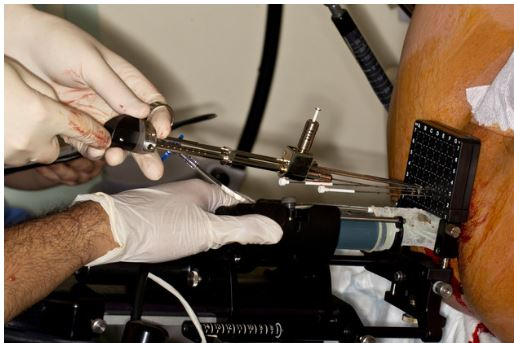
\includegraphics[width=0.5\textwidth]{Imagens/aplicadorMick.JPG}
					\caption{Aplicador MICK utilizado na Braquiterapia de próstata. São utilizadas agulhas para inserção das fontes.}
					\label{img:aplicadorMick}
				\end{figure}

				\item Os aplicadores permitem que a fonte permaneça em uma posição fixa durante todo o tratamento. \textit{\textcolor{CarnationPink}{Exemplo:}} \textit{Sonda e ovóides, Figura \ref{img:aplicadorSondaEOvoides}.}
				
				\begin{figure}[h]
					\centering
					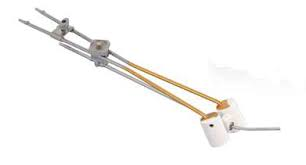
\includegraphics[width=0.5\textwidth]{Imagens/aplicadorSondaEOvoides.jpg}
					\caption{Aplicador ginecológico com sonda e ovóides.}
					\label{img:aplicadorSondaEOvoides}
				\end{figure}
			\end{enumerate}

			Os tipos de carregamento podem ser definidos com base na forma que as fontes serão inseridas e de acordo com o tempo com que a fonte ficará em cada posição de parada.

			Quanto a forma de inserção, o carregamento da fonte pode ser classificado como:

			\begin{itemize}
				\item \textbf{Braquiterapia com pré-carregamento manual (\textit{preloaded}):} Onde as fontes são pré-carregadas no aplicador antes de ser inserido no paciente.
				\item \textbf{Braquiterapia com pós-carregamento manual (\textit{Manually afterloaded}):} Os aplicadores são inseridos no paciente e na sequência o médico insere manualmente as fontes nos aplicadores.
				\item \textbf{Braquiterapia com pós-carregamento remoto (\textit{Remotely afterloaded}):} O aplicador é inserido no paciente e um equipamento é responsável por mover as fontes dentro do aplicador de acordo com as posições remotamente pré-definidas. Neste procedimento é envolvida uma maior tecnologia que permite uma maior precisão no posicionamento das fontes.
			\end{itemize}

			Já com base distribuição dos tempos de parada das fontes, o carregamento pode ser definido como:

		% Completar aqui o motivo dos carregamentos serem diferentes e a mudança na distribuição de dose
			\begin{itemize}
				\item \textbf{Carregamento Uniforme: } Onde as fontes com a mesma atividade permanecerão o mesmo período de tempo em cada posição de parada.
				\item \textbf{Carregamento Não-Uniforme:} As fontes permanecem tempos diferentes em cada posição de parada. 
			\end{itemize}
		
	\section{Radioatividade}

		A Radioatividade é o fenômeno físico por trás das emissão de radiação pelas fontes utilizadas em braquiterapia. Os principais relações físicas da Radioatividade são:

		\begin{itemize}
			\item \textbf{Desintegração por unidade de tempo:} Mostra o número de átomos que se desintegram com o passar do tempo. 

				\begin{equation}
					\frac{dN}{dt} = -\lambda N
					\label{eq:DesintegraçãoPorUnidadeDeTempo}
				\end{equation}
		
				onde, 

				$\frac{dN}{dt}$ é o número de desintegrações por unidade de tempo;

				$\lambda$ é a constante de decaimento; e

				$N$ é o número de átomos radioativos da amostra.

				O sinal negativo na equação indica que o número de átomos radioativos remanescentes na amostra diminui com o passar do tempo. 

			\item \textbf{Lei do decaimento exponencial: } Permite obter o número de átomos radioativos em  um tempo t qualquer que ainda não decaíram.

				\begin{equation}
					N(t) = N_0 \times e^{-\lambda t}
					\label{eq:decaimentoExponencial}
				\end{equation}
				
				onde,

				$N_0$ é o número inicial de átomos radioativos (t = 0);
				
				$t$ é o tempo decorrido; e

				$N(t)$ é a quantidade de átomos radioativos remanescentes após um tempo t.

				Através da Equação \ref{eq:decaimentoExponencial} podemos extrair que a fração de átomos que permanecem na amostra após um tempo t é dada por 

				\begin{equation}
					\frac{N(t)}{N_0}
				\end{equation}

				E a fração de átomos que decaíram da amostra é dada por:

				\begin{equation}
					1 - \frac{N(t)}{N_0}
				\end{equation}

			\item \textbf{Tempo de meia-vida ($t_{1/2}$): } É o tempo no qual o número de átomos radioativos de uma amostra demora para decair pela metade do seu valor inicial, ou seja o número de átomos radioativos remanescentes na amostra fique igual a metade do seu valor inicial, 
			
				\begin{equation}
					N(t) = {1/2}N_0
				\end{equation}

				Portanto o tempo de meia-vida  ($t_{1/2}$) é dado por:

				\begin{equation}
					t_{1/2} = \frac{\ln 2}{\lambda}
				\end{equation}

				\textbf{\textcolor{CarnationPink}{Obs:} } Podemos notar que um material radioativo com uma vida longa está relacionado com um grande tempo de veia vida e portanto um pequeno valor para a taxa de decaimento.

				Após $n$ $t_{1/2}$ temos que:

				\begin{equation}
					N = \left({1/2}\right)^n N_0
				\end{equation}



% Deduzir o porque a vida média assume que N é igual a 1/e				
			\item \textbf{Tempo de vida-média ($\tau$): } Se caracteriza como o tempo necessário para que todos os átomos radioativos decaiam assumindo que a taxa de decaimento se mantenha fixa em seu valor inicial.
			
				\begin{equation}
					\tau = \frac{1}{\lambda}
				\end{equation}

				\begin{equation}
					\tau = 1.44 \times t_{1/2}
				\end{equation}

				\textbf{\textcolor{CarnationPink}{Obs:} } O tempo de vida média é utilizado para calcular a dose total recebida em um implante permanente pois as fontes radioativas ficarão em todo o seu tempo de vida inseridas no paciente e a vida média descreve o tempo médio total que um material permanece radioativo.

			\item \textbf{Meia Vida Biológica ($t_{biol}$): } É o tempo que leva para a metade da fonte ser eliminada pelo próprio corpo.
			
			\item \textbf{Meia Vida Efetiva ($t_{eff}$): } É o tempo de meia vida que considera tanto a eliminação biológica do material quanto o seu tempo de decaimento.
			
				\begin{equation}
					\frac{1}{t_{eff}} = \frac{1}{t_{1/2}} + \frac{1}{t_{biol}}
				\end{equation}

			\item \textbf{Atividade ($A$): } É definida como o número de desintegrações por unidade de tempo, ou seja, é a taxa de decaimento de uma fonte radioativa. 
				
				\begin{equation}
					A = -\frac{dN}{dt} = \lambda N
				\end{equation}

			\item \textbf{Atividade em função do tempo ($A(t)$): } Uma vez conhecida a atividade $A_0$ em um tempo $t_0$ qualquer, pode-se obter a atividade da fonte em função do tempo, seja ele no passado ou futuro através da equação:
				
				\begin{equation}
					A(t) = A_0 \times e^{-\lambda t}
					\label{eq:AtividadeNoTempo}
				\end{equation}

			\item \textbf{Atividade Específica: } É definida como a atividade de um material por unidade de massa. É uma grandeza importante para a produção de fontes de braquiterapia HDR,pois uma alta atividade específica fornece uma maior atividade em uma menor quantidade de material radioativo, permitindo uma alta taxa de dose em uma fonte pequena o suficiente para ser inseridas nas cavidades onde ocorrerá o tratamento.

		\end{itemize}

	\section{Especificação da Fonte}
		
		Uma fonte pode ser especificada com base na determinação da força da fonte \textit{(Source Strength)}. Essa grandeza sofreu variações ao longo do tempo, de acordo com o surgimento de novas fontes de radiação que substituíram o Rádio-226. 

		\subsection{Massa de Radio-226}

			Forma antiga de especificação da fonte que se baseia na quantidade de material presente na amostra. Era expressa em $mg\; Ra$ que quantificava a quantidade de radiação emitida quando a única fonte de radiação utilizada em braquiterapia era o $\mathrm{{}^{226}Ra}$

		\subsection{Massa de Rádio Equivalente}

			Foi introduzida quando surgiram diferentes materiais radioativos para serem utilizados em braquiterapia, como o Césio-137 (${}^{137}Cs$). Esta quantidade é definida como a massa de Rádio, encapsulada em 0.5 mm de Platina (Pt) que produz a mesma taxa de exposição da fonte de interesse na posição de calibração.

		\subsection{Atividade}

			É uma das grandezas que pode ser utilizada para especificar a fonte. Como descrito anteriormente, a Atividade é definida como o número de núcleos se submetendo ao decaimento radioativo por unidade de tempo, Equação \ref{eq:AtividadeNoTempo}.

			\begin{itemize}
				\item Unidade SI: \textbf{Bq} (Becquerel) = $1\;dps$
				\item Unidade Antiga: \textbf{Ci} (Curie) = $3.7 \times 10^{10}\; Bq$
			\end{itemize}

			\textbf{\textbf{\textcolor{CarnationPink}{Obs:} } }Embora não ser a unidade oficial do SI, o \textbf{Ci} ainda é muito utilizado na rotina clínica. \textit{\textbf{\textcolor{CarnationPink}{Exemplo:}}} \textit{O Irídio-192 utilizado em tratamentos HDR possui atividade típica entre 5 Ci e 10 Ci}

		\subsection{Atividade Aparente}

			Este conceito considera a filtragem da radiação emitida que ocorre devido ao encapsulamento da fonte. Toda fonte de radiação é revestida por um metal que absorve parte da radiação emitida. Portanto, a Atividade Aparente é definida como a atividade de uma fonte pontual hipotética, não filtrada, que tem a mesma taxa de exposição na distância de calibração da fonte de interesse. Como a exposição de uma fonte é menor, devido ao encapsulamento, esta grandeza relaciona-se com a atividade que irá causar essa mesma taxa de exposição se não houvesse a blindagem.
	

		
		\subsection{Taxa de Exposição}

			A taxa de Exposição é definida como a taxa pelo o qual o ar é ionizado pela radiação indiretamente ionizante (\textbf{\textit{\textcolor{CarnationPink}{raios-$\gamma$}}}). É portanto a taxa de carga produzida no ar pela radiação indiretamente ionizante por unidade de massa de ar.

			\begin{itemize}
				\item Unidade SI: $C/Kg\cdot h$
				\item Unidade Antiga: $R / h$
			\end{itemize}

			A relação entre o Roentgen e A Unidade do SI é obtida pela seguinte relação:

			\begin{equation}
				1\;R = 2.58 \times 10^{-4}\; \frac{C}{Kg}
			\end{equation}

			\textbf{\textcolor{CarnationPink}{Obs:} } Normalmente a força da fonte de um emissor gama é determinado em termos da taxa de exposição em uma distância de calibração de 1 m da fonte.

			A uma distância específica da fonte, a taxa de exposição (\textbf{\textit{\textcolor{CarnationPink}{$\dot{X}$}}}) está relacionada com a Atividade de uma fonte através da constante de taxa de exposição $\Gamma$.

				\begin{equation}
					\Gamma = \frac{\dot{X}(r)}{A} \cdot r^2
				\end{equation}

				onde, 

				$r$ é a distância entre a fonte e o ponto de análise.

		\subsection{Força kerma-ar}

			É uma unidade desenvolvida pela AAPM para especificar a força da fonte de emissores gama. 

			\begin{itemize}
				\item \textbf{Kerma}: quantifica a energia que foi transferida para as partículas carregadas por unidade de massa em um volume do meio;
				\item \textbf{Força kerma-ar \textbf{\textit{\textcolor{CarnationPink}{$S_k$}}} }: É a medida da energia transferida para o ar.
			\end{itemize}

			$S_k$ é definido como o produto da taxa kerma-ar medido em uma distância $d$ específica, a partir do centro da fonte ao longo do seu eixo transversal, multiplicado pelo quadrado da distância.

			\begin{equation}
				S_k = \dot{K}(d) \cdot d^2
			\end{equation}

			\textbf{\textcolor{CarnationPink}{Obs:} } $S_k$ é medido no ar livre, normalmente a 1 m de distancia do centro da fonte.

			\

			A unidade no SI para a Força kerma-ar é \textbf{\textcolor{CarnationPink}{U}}, onde


			\begin{equation}
				U = cGy \cdot cm^2 / h = \mu Gy \cdot m^2 / h
			\end{equation}

	\section{Fontes Utilizadas Em Braquiterapia}
			
		\subsection{Rádio 226 \textbf{\textcolor{CarnationPink}{(${}^{226}Ra$)}}}
			
			
			\begin{itemize}
				\item \textbf{Aplicação Clínica:} LDR Intracavitária e Intersticial
				\item \textbf{Sítios de tratamento mais comuns:} Historicamente utilizada
				\item \textbf{Forma da fonte:} Tubos e agulhas
				\item \textbf{Partícula Emitida:} Raios-$\gamma$
				\item \textbf{Energia média: } 830 KeV
				\item \textbf{HVL:} 12 mm de Pb
				\item \textbf{$t_{1/2}$:} 1600 anos
				\item \textbf{\% de mudança de atividade: } 0.04\% ao ano
			\end{itemize}

			\
		
		\subsection{Césio 137 \textbf{\textcolor{CarnationPink}{(${}^{137}Cs$)}}}

			\begin{itemize}
				\item \textbf{Aplicação Clínica:} LDR Intracavitária e Intersticial
				\item \textbf{Sítios de tratamento mais comuns:} Cervix e útero
				\item \textbf{Forma da fonte:} tubos e agulhas
				\item \textbf{Partícula Emitida:} Raios-$\gamma$
				\item \textbf{Energia média: } 662 KeV
				\item \textbf{HVL:} 5.5 mm Pb
				\item \textbf{$t_{1/2}$:} 30 anos
				\item \textbf{\% de mudança de atividade: } 2.3\% por dia
			\end{itemize}

			\

		\subsection{Cobalto 60 \textbf{\textcolor{CarnationPink}{(${}^{60}Co$)}}}
		


			\begin{itemize}
				\item \textbf{Aplicação Clínica:} LDR Intracavitária e Intersticial e HDR Intracavitária
				\item \textbf{Sítios de tratamento mais comuns:} Multiplos sítos
				\item \textbf{Forma da fonte:} fio
				\item \textbf{Partícula Emitida:} Raios-$\gamma$
				\item \textbf{Energia média: } 1250 KeV
				\item \textbf{HVL:} 11 mm de Pb
				\item \textbf{$t_{1/2}$:} 5.26 anos
				\item \textbf{\% de mudança de atividade: } 12.3\% ao ano.
			\end{itemize}

			\

		\subsection{Ouro 198 \textbf{\textcolor{CarnationPink}{(${}^{198}Au$)}}}


			\begin{itemize}
				\item \textbf{Aplicação Clínica:} LDR intersticial
				\item \textbf{Sítios de tratamento mais comuns:} Próstata
				\item \textbf{Forma da fonte:} Sementes
				\item \textbf{Partícula Emitida:} Raios-$\gamma$
				\item \textbf{Energia média: } 412 KeV
				\item \textbf{HVL:} 2.5 mm de Pb
				\item \textbf{$t_{1/2}$:} 2.7 dias
				\item \textbf{\% de mudança de atividade: } 22.6\% por dia
			\end{itemize}

			\

		\subsection{Irídio 192 \textbf{\textcolor{CarnationPink}{(${}^{192}Ir$)}}}

			\begin{itemize}
				\item \textbf{Aplicação Clínica:} HDR Intracavitária, Intersticial e Superficial e LDR intersticial
				\item \textbf{Sítios de tratamento mais comuns:} Cervix, útero, sarcomas, cabeça e pescoço, prostata e mama.
				\item \textbf{Forma da fonte:} Sementes, fios e fitas
				\item \textbf{Partícula Emitida:} Raios-$\gamma$
				\item \textbf{Energia média: } 380 KeV
				\item \textbf{HVL:} 2.5 mm de Pb
				\item \textbf{$t_{1/2}$:} 73.8 dias
				\item \textbf{\% de mudança de atividade: } 0.9\% por dia
			\end{itemize}

			\

		\subsection{Iodo 125 \textbf{\textcolor{CarnationPink}{(${}^{125}I$)}}}

			\begin{itemize}
				\item \textbf{Aplicação Clínica:} LDR Intersticial e Superficial
				\item \textbf{Sítios de tratamento mais comuns:} Próstata e olho
				\item \textbf{Forma da fonte:} sementes
				\item \textbf{Partícula Emitida:} Raios-$\gamma$
				\item \textbf{Energia média: } 28 KeV
				\item \textbf{HVL:} 0.025 mm de Pb
				\item \textbf{$t_{1/2}$:} 59.4 dias
				\item \textbf{\% de mudança de atividade: } 1.2\% por dia
			\end{itemize}

			\

		\subsection{Paládio 103 \textbf{\textcolor{CarnationPink}{(${}^{103}Pd$)}}}


			\begin{itemize}
				\item \textbf{Aplicação Clínica:} LDR Intersticial
				\item \textbf{Sítios de tratamento mais comuns:} Próstata
				\item \textbf{Forma da fonte:} Sementes
				\item \textbf{Partícula Emitida:} Raios-$\gamma$
				\item \textbf{Energia média: } 21 KeV
				\item \textbf{HVL:} 0.008 mm de Pb
				\item \textbf{$t_{1/2}$:} 17 dias
				\item \textbf{\% de mudança de atividade: } 4.0\% por dia
			\end{itemize}

			\
		
		\subsection{Césio 131 \textbf{\textcolor{CarnationPink}{(${}^{131}Cs$)}}}

			\begin{itemize}
				\item \textbf{Aplicação Clínica:} LDR Intersticial
				\item \textbf{Sítios de tratamento mais comuns:} Próstata
				\item \textbf{Forma da fonte:} Sementes
				\item \textbf{Partícula Emitida:} Raios-$\gamma$
				\item \textbf{Energia média: } 29 KeV
				\item \textbf{HVL:} 0.025 mm de Pb
				\item \textbf{$t_{1/2}$:} 9.7 dias
				\item \textbf{\% de mudança de atividade: } 6.9\% por dia
			\end{itemize}

			\

		\subsection{Estrôncio 90 \textbf{\textcolor{CarnationPink}{(${}^{90}Sr$)}}}

			\begin{itemize}
				\item \textbf{Aplicação Clínica:} LDR Superficial
				\item \textbf{Sítios de tratamento mais comuns:} Olhos
				\item \textbf{Forma da fonte:} Sementes, placas ou aplicadores
				\item \textbf{Partícula Emitida:} partícula-$\beta$
				\item \textbf{Energia média: } 224 KeV (máxima)
				\item \textbf{HVL:} N/A
				\item \textbf{$t_{1/2}$:} 28.8 anos
				\item \textbf{\% de mudança de atividade: } 2.4\% por dia
			\end{itemize}

	
	\section{Distribuição de Dose em Braquiterapia}

		Devido a baixa energia dos fótons emitidos por fontes de braquiterapia, que é da ordem de KeV, a distribuição de dose apresenta um alto gradiente de dose e um falloff de dose mais rápido quando comparado à teleterapia.

		A maior vantagem deste gradiente acentuado é conseguir poupar os tecidos sadios adjacentes.Porém, caso o alvo esteja distante da fonte, cobrir o alvo com a dose de prescrição será difícil pelo mesmo motivo, pois irá aumentar a dose nos tecidos mais próximos. Portanto para diminuir a dose em volta do alvo indica-se utilizar o maior aplicador possível para que este tecido seja afastado para longe da fonte em uma região com um menor gradiente de dose. 

		Uma discrepância de milímetros em braquiterapia pode ser crítica no tratamento devido à forma do falloff de dose e portanto requer uma precisão milimétrica no posicionamento da fonte em sistemas afterloading.

		\begin{figure}
			\centering
			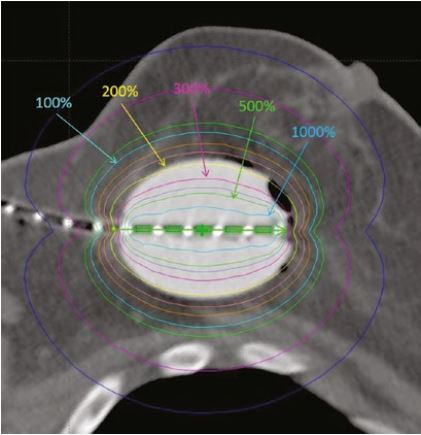
\includegraphics[width=0.5\textwidth]{Imagens/falloffDoseMammosite.JPG}
			\caption{Distribuição de dose com um balão de mama inflado. A dose de prescrição está a 1 cm de profundidade da superfície do balão. Caso o balão seja esvaziado, a dose nesse mesmo ponto pode ficar 10 vezes maior que a dose de prescrição.}
		\end{figure}

		São 3 fatores que impactam na forma da distribuição de dose em braquiterapia: \textbf{\textcolor{CarnationPink}{distância da fonte, forma e encapsulamento e o material do encapsulamento}}.

		\begin{enumerate}
			\item Para distancias grandes da fonte, ou seja, para distancias de no mínimo duas vezes o tamanho da fonte, a distribuição de dose é governada pela \textbf{\textcolor{CarnationPink}{lei do inverso quadrado}}. Porém, quanto mais próximo está o ponto de análise da fonte, menos aplicável é a lei do inverso quadrado.
			
			\item A forma cilíndrica da fonte faz com que a dose ao longo do seu eixo longitudinal seja diminuída devido a penetração em uma maior quantidade de material quando comparado ao eixo axial, causando uma maior filtração da radiação nessa direção. A Figura \ref{img:distribuicaoDeDose} mostra o comportamento da distribuição de dose ao longo do eixo longitudinal da fonte.
			
				\begin{figure}[h]
					\centering
					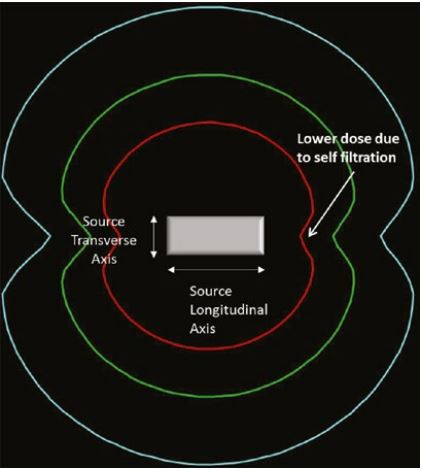
\includegraphics[width=0.5\textwidth]{Imagens/distribuicaoDeDose.JPG}
					\caption{Distribuição de dose na água para uma fonte realística de $\mathrm{{}^{192}Ir}$}
					\label{img:distribuicaoDeDose}
				\end{figure}

			\item O material do encapsulamento está diretamente relacionado à absorção e ao espalhamento dos fótons causando uma atenuação dos fótons emitidos.
		\end{enumerate}
	
	\section{Métodos de Cálculo de Dose}

		Existem diferentes métodos para obtenção da Dose envolvida em procedimentos de braquiterapia. 

		\subsection{Cálculos de Dose Cumulativa}

			São utilizados para determinar a dose total entregue ao longo de todo o período de tratamento. Como a atividade muda com o decorrer do tempo, a taxa de dose também muda com o decorrer do tempo e pode ser obtida através da seguinte relação:

				\begin{equation}
					\dot{D}(t) = \dot{D_0} e^{-\lambda t}
					\label{eq:taxaDeDose}
				\end{equation}

			onde,

			$\dot{D_0}$ é a taxa de dose inicial da amostra.

			A dose total acumulada em um tempo específico pode ser obtida integrando a Equação \ref{eq:taxaDeDose} no tempo t, ou seja:

				\begin{equation}
					D(t) = \int_{t_0}^{t} \dot{D_0} e^{-\lambda t}\,dt
					\label{eq:integralDaDose}
				\end{equation}

			Resolvendo a integral apresentada na Equação \ref{eq:integralDaDose}, obtemos a relação que nos fornece a dose acumulada após um tempo t (dose total).

				\begin{equation}
					D(t) = \frac{1}{\lambda} \; \dot{D_0} \; (1 - e^{-\lambda t})
					\label{eq:doseCumulativa}
				\end{equation}

			Sabendo que $$\frac{1}{\lambda} = \tau = 1.44 t_{1/2}$$ A equação \ref{eq:doseCumulativa} pode ser escrita da forma:

				\begin{equation}
					D(t) = 1.44\,t_{1/2} \,\dot{D_0} (1 - e^{-\lambda t})
				\end{equation}

			No caso de implantes permanentes cuja meia vida do elemento é curta, o tempo de tratamento será muito maior que o tempo de meia vida deste elemento pois a dose será entregue ao longo de toda a vida da fonte. Podemos fazer então uma aproximação na Equação \ref{eq:doseCumulativa} quando $t >> t_{1/2}$: 

			Como $$t >> t_{1/2}$$ então $$\frac{t}{t_{1/2}} >> 1$$

			Como $$\lambda = \frac{ln 2}{t_{1/2}}$$ Substituindo este valor na Equação \ref{eq:doseCumulativa} temos que: 

			$$ D(t) = \frac{1}{\lambda}  \; \dot{D_0} \; \left(1 - e^{-\frac{ln 2}{t_{1/2}} t}\right) $$

			$$D(t) = \frac{1}{\lambda}  \; \dot{D_0} \; \left(1 - \frac{1}{e^{ln 2 \frac{t}{t_{1/2}}}}\right)$$

			Avaliando no limite quando $\frac{t}{t_{1/2}} \rightarrow \infty$ temos:

			$$ \lim_{{\frac{t}{t_{1/2}}} \to \infty} D(t) = \lim_{{\frac{t}{t_{1/2}}} \to \infty} \frac{1}{\lambda}  \; \dot{D_0} \; \left(1 - \frac{1}{e^{ln 2 \frac{t}{t_{1/2}}}}\right)$$

			Aplicando as propriedades de limite temos

			$$\lim_{{\frac{t}{t_{1/2}}} \to \infty} D(t) = \frac{1}{\lambda} \; \dot{D_0} \;  \left(\lim_{{\frac{t}{t_{1/2}}} \to \infty} 1 - \lim_{{\frac{t}{t_{1/2}}} \to \infty} \frac{1}{e^{ln 2 \frac{t}{t_{1/2}}}}\right)$$

			Como $1/ \lambda$ e $\dot{D_0}$ são constantes e:

			$$\lim_{{\frac{t}{t_{1/2}}} \to \infty} 1 = 1$$

			$$\lim_{{\frac{t}{t_{1/2}}} \to \infty} \frac{1}{e^{ln 2 \frac{t}{t_{1/2}}}} = \frac{1}{e^{\infty}} = 0 $$

			Chegamos na equação de dose total quando $t >> t_{1/2}$:

			\begin{equation}
				D = \frac{1}{\lambda} \; \dot{D_0} = \tau \; \dot{D_0} = 1.44 \; t_{1/2} \; \dot{D_0}
				\label{eq:aproximacaoImplantesPermanentes}
			\end{equation}


			Outro caso a ser avaliado, são em implantes temporários cujo tempo de exposição é muito menor que o tempo de meia vida da fonte radioativa. Podemos fazer então uma aproximação da dose total para os casos em que $t << t_{1/2}$. 


			Como $t << t_{1/2}$, então

			$$\frac{t}{t_{1/2}} << 0 $$

			Podemos então utilizar a série de taylor para expandir o termo da exponencial. 

			Para $x << 0$

			$$e^x = 1 + x + \frac{x^2}{2!} + \frac{x^3}{3!} + \dots$$

			Truncando a série na primeira ordem, pois os termos quadráticos são ínfimos, temos que

			$$ e^{-ln 2 \frac{t}{t_{1/2}}} = 1 - ln 2 \; \frac{t}{t_{1/2}}$$

			Substituindo na equação \ref{eq:doseCumulativa} temos então

			$$D(t) = \frac{1}{\lambda} \; \dot{D_0} \; \left[1 - \left(1 - \ln 2 \; \frac{t}{t_1/2}\right)\right]$$

			Fazendo as devidas simplificações, chegamos na equação para a dose total quando $t << t_{1/2}$

			\begin{equation}
				D(t) = \dot{D_0} \; t
				\label{eq:AproximacaoImplantesTemporarios}
			\end{equation}

			Portanto a Dose total é dada pela multiplicação da taxa de dose inicial pelo o tempo de tratamento, o que faz sentido pois a atividade de uma fonte com o tempo de meia-vida muito maior que o tempo de tratamento, não sofrerá mudanças significativas nesse curto espaço de tempo.


			Nos casos em que o tempo de tratamento é da ordem do tempo de meia vida da fonte, haverá uma mudança signicativa da Atividade durante o tempo de tratamento, então a dose total é obtida através da Equação \ref{eq:doseCumulativa}.

		\subsection{Método de Integral e Interpolação}

			Foram métodos Historicamente utilizados para os cálculos de dose em fontes com formatos tubulares ou em forma de sementes.

			O método \textbf{\textcolor{CarnationPink}{Integral de Sievert}} subdivide a fonte em n partes iguais. As partes são divididas em partes pequenas o suficiente de forma que possam ser consideradas como fontes pontuais. Para um determinado ponto próximo a fonte, a dose é determinada somando às contribuições das n partes considerando os fatores de correção aplicados separadamente para cada parte. Os fatores de correção utilizados são: \textit{fator distância, filtração obliqua, atenuação e espalhamento}.

			O \textbf{\textcolor{CarnationPink}{Método de Interpolação}} utiliza tabelas de dados de conjuntos de pontos que foram previamente obtidos através de técnicas experimentais ou de modelos teóricos. As tabelas \textit{\textcolor{CarnationPink}{along-and-away}} foram muito utilizadas para tratamentos com $\mathrm{{}^{137}Cs}$ e dados tabelados também foram muito utilizados nos sistemas Paterson-Parker e Quimbly.

		\subsection{Formalismo Modular: TG-43}

			É o método padrão para cálculos de taxa de dose 1D e 2D. Este método assume uma fonte cilíndrica simétrica considerando às diferenças na distribuição de dose causadas pela forma da fonte. A dose obtida nesse formalismo é determinada para um meio homogêneo de água e portanto não considera a heterogeneidade do meio. Os dados deste formalismo foram obtidos através de medidas experimentais e através de simulações de Monte-Carlo para fontes conhecidas, que é utilizado nos sistemas de planejamento.

			Este método é dividido em módulos onde cada parâmetro depende da posição do ponto de cálculo de dose com respeito à fonte. A Figura \ref{img:FormalismoTg43} mostra a geometria utilizada para cálculo da distribuição de dose. A posição do ponto de cálculo é dada em coordenadas polares $\mathrm{P(r, \theta)}$ onde $r$ é a distância radial do ponto até o centro da fonte e $\theta$ é o ângulo formado com o eixo longitudinal da fonte (eixo z na figura) tomado a partir centro da fonte. A posição $\mathrm{P_0(r_0, \theta_0)}$ é a posição de referência dos cálculos localizada radialmente a 1 cm da fonte ($r_0 = 1 \; cm$) ao longo do eixo central da fonte (eixo y na figura) fazendo um ângulo $\theta_0 = \pi / 2$ com o eixo longitudinal da fonte.


				\begin{figure}[h]
					\centering
					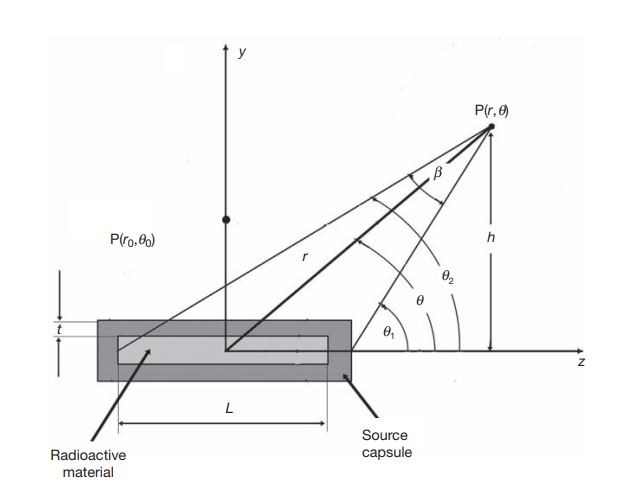
\includegraphics[width=0.8\textwidth]{Imagens/esquemaFormalismoTg43.JPG}
					\caption{Geometria Utilizada para determinação da taxa de dose no Formalismo do TG 43}
					\label{img:FormalismoTg43}
				\end{figure}

			A taxa de dose em função da posição do ponto de cálculo é dada por:

			\begin{equation}
				\dot{D}(r, \theta) = S_k \; \varLambda \; \frac{G(r, \theta)}{G(r_0, \theta_0)} 
				\; g(r) \; F(r, \theta)
				\label{eq:formalismoTg43}
			\end{equation}

			onde:

			\begin{itemize}
				\item \textbf{\textcolor{CarnationPink}{$\varLambda$} : } é a constante de taxa de dose responsável por corrigir a medida no ar para a água. É definida como a taxa de dose na água por unidade de força Kerma-ar na posição de referência $\mathrm{P_0(r_0, \theta_0)}$.
					$$[\varLambda] = cGy / U \cdot h$$

				\item \textbf{\textcolor{CarnationPink}{$S_k$} : } É a força Kerma-ar. É definida como a taxa kerma-ar medida em uma distância específica do centro da fonte ao longo do seu eixo transversal multiplicado pelo quadrado da distância do ponto à fonte, medida no ar livre.

					\begin{equation}
						S_k = \dot{K}(d) \cdot d^2
					\end{equation}

					$$[S_k] = U = cGy \cdot cm^2 / h$$

				\item \textbf{\textcolor{CarnationPink}{$G(r, \theta)$}: } É a função Geométrica. Fornece a efetiva lei do inverso quadrado pois considera a variação da dose relativa devido à distribuição espacial da atividade dentro da fonte (forma da fonte). Depende apenas da distância radial e angular do ponto de análise portanto não considera o espalhamento e a atenuação da fonte.
				
					$$[G(r_ \theta)] = cm^{-2}$$

					Para uma fonte Pontual:

					\begin{equation}
						G(r, \theta) = \frac{1}{r_2}
					\end{equation}

					Para uma fonte cilíndrica:

					\begin{equation}
						G(r, \theta) = \frac{\beta}{L \; r \; sen(\theta)}, \qquad para \qquad \theta \neq 0
					\end{equation}

					\begin{equation}
						G(r, \theta) = \left(r^2 - \frac{L^2}{4}\right)^{-1}, \qquad para \qquad \theta = 0
					\end{equation}
				
				\item \textbf{\textcolor{CarnationPink}{$g(r)$} : } É chamada de Função de dose radial. É uma quantidade adimensional que considera o falloff da dose ao longo do plano transversal da fonte devido ao espalhamento e a atenuação no material do encapsulamento da fonte. É definida ao longo do eixo transversal $\mathrm{(\theta = \pi / 2)}$, portanto depende apenas da distância radial do ponto à fonte.
				
					Na distância de referência $r_0$

					$$g(r_0) = 1$$
				
				\item \textbf{\textcolor{CarnationPink}{$F(r, \theta)$} : } É chamada de Função de Anisotropia. Leva em consideração o formato anisotrópico da distribuição de dose causado pela própria filtração do encapsulamento da fonte e a transmissão oblíqua através do encapsulamento. Fonece a distribuição de dose para ângulos diferentes de $\theta = \pi / 2$, ou seja, para pontos em ângulos fora do eixo transversal da fonte.
				
					Para $\theta = \theta_0 = \pi/2$

					$$F(r, \theta_0) = 1$$

			\end{itemize}

			

	\bibliography{ref.bib}

\end{document}